\documentclass[12pt,a4paper]{article}

\usepackage{fontspec}
\usepackage{polyglossia}
\setmainlanguage{polish}
\setmainfont{Latin Modern Roman}

\usepackage[a4paper,left=2.15cm,right=2.15cm,top=2.05cm,bottom=2.15cm]{geometry}
\usepackage{amsmath,amssymb}
\usepackage{graphicx}
\usepackage{array}
\usepackage{booktabs}
\usepackage{caption}
\usepackage{subcaption}
\usepackage{float}
\usepackage{hyperref}
\usepackage{indentfirst}
\usepackage{ragged2e}

\hypersetup{hidelinks}
\captionsetup{font=small,labelformat=empty,justification=centering}
\setlength{\parindent}{1.15cm}
\setlength{\parskip}{0pt}
\renewcommand{\arraystretch}{1.15}

\newcommand{\chaptertitle}[1]{\section*{#1}\addcontentsline{toc}{section}{#1}}
\newcommand{\subchaptertitle}[1]{\subsection*{#1}\addcontentsline{toc}{subsection}{#1}}
\newcommand{\figcaption}[1]{\caption*{\small #1}}
\newcommand{\twopanel}[4]{%
  \begin{figure}[H]\centering
    \begin{minipage}{0.48\textwidth}\centering
      \includegraphics[width=\linewidth]{#1}\\[-0.2em]a)
    \end{minipage}\hfill
    \begin{minipage}{0.48\textwidth}\centering
      \includegraphics[width=\linewidth]{#2}\\[-0.2em]b)
    \end{minipage}
    \figcaption{#3 #4}
  \end{figure}
}

\begin{document}
\pagestyle{plain}

\begin{titlepage}
\thispagestyle{empty}
\centering
{\large Uniwersytet Warszawski\\
Wydział Fizyki\par}
\vspace{1.4cm}
{\large Bartosz Wieciech\\
nr albumu: 276965\par}
\vspace{3.0cm}
{\Large\itshape Modelowanie propagacji światła w nanostrukturach fotonicznych\\
metodą elementów skończonych\par}
\vspace{1.7cm}
{\large Praca licencjacka\\
na kierunku inżynieria nanostruktur\\
z zakresu fotoniki\par}
\vfill
\begin{flushright}
Praca wykonana pod kierunkiem\\
dr hab. Rafała Kotyńskiego\\
Zakład Optyki Informacyjnej
\end{flushright}
\vspace{1.6cm}
Warszawa, wrzesień 2014
\end{titlepage}

\setcounter{page}{2}
\mbox{}
\newpage

\chaptertitle{Oświadczenie kierującego pracą}

Oświadczam, że niniejsza praca została przygotowana pod moim kierunkiem i stwierdzam, że
spełnia ona warunki do przedstawienia jej w postępowaniu o nadanie tytułu zawodowego.

\vspace{1.5cm}
\noindent Data\hspace{3.5cm}Podpis kierującego pracą

\vspace{2.0cm}
\chaptertitle{Oświadczenie autora pracy}

Świadom odpowiedzialności prawnej oświadczam, że niniejsza praca dyplomowa została napisana
przeze mnie samodzielnie i nie zawiera treści uzyskanych w sposób niezgodny z obowiązującymi
przepisami.

Oświadczam również, że przedstawiona praca nie była wcześniej przedmiotem procedur
związanych z uzyskaniem tytułu zawodowego w wyższej uczelni.

Oświadczam ponadto, że niniejsza wersja pracy jest identyczna z załączoną wersją elektroniczną.

\vspace{1.5cm}
\noindent Data\hspace{3.5cm}Podpis autora pracy

\newpage
\mbox{}
\newpage

\chaptertitle{Streszczenie}

Zastosowano metodę elementów skończonych do modelowania rozchodzenia się światła w
periodycznych nanostrukturach fotonicznych. Rozwiązywano w tym celu dwuwymiarowe
wektorowe równanie falowe. Symulacje wykonano dla kryształów fotonicznych o różnej strukturze
sieci, do których wprowadzono defekty liniowe. Przedstawiono różnice wynikające z zastosowania
fal o różnych częstościach, leżących wewnątrz fotonicznej przerwy wzbronionej układu, jak i poza
nią. Wykonano symulację prowadzenia modu zlokalizowanego w defekcie liniowym kryształu
fotonicznego. Badano również transmisję promieniowania elektromagnetycznego przez siatki
dyfrakcyjne o podwójnej periodyczności. Modelowanie przeprowadzono dla układów wykonanych
ze srebra, złota, chromu oraz idealnego przewodnika, dla długości fali 400 nm.

\vspace{1.2cm}
\chaptertitle{Słowa kluczowe}

Metoda elementów skończonych, modelowanie elektromagnetyczne, PML, światło, wektorowe
równanie falowe, kryształ fotoniczny, fotoniczna przerwa wzbroniona, siatka podfalowa

\vspace{1.2cm}
\chaptertitle{Dziedzina pracy (kody wg programu Socrates-Erasmus)}

[13.2] Fizyka

\vspace{1.2cm}
\chaptertitle{Tytuł pracy w języku angielskim}

Modeling of light propagation in photonic nanostructures using the finite element method

\newpage
\mbox{}
\newpage

\chaptertitle{Spis treści}
\begingroup\small
\noindent Rozdział 1. Wstęp\dotfill 8\\
Rozdział 2. Wprowadzenie teoretyczne\dotfill 9\\
\hspace*{1em}2.1. Równania Maxwella i dwuwymiarowe wektorowe równanie falowe\dotfill 9\\
\hspace*{1em}2.2. Metoda elementów skończonych\dotfill 11\\
\hspace*{1em}2.3. Równanie różniczkowe typu eliptycznego i metoda jego przybliżonego rozwiązywania\dotfill 12\\
\hspace*{1em}2.4. Warunki brzegowe PML\dotfill 13\\
\hspace*{1em}2.5. Kryształy fotoniczne\dotfill 15\\
\hspace*{1em}2.6. Siatki dyfrakcyjne\dotfill 16\\
Rozdział 3. Wyniki symulacji\dotfill 18\\
\hspace*{1em}3.1. Propagacja światła w kryształach fotonicznych\dotfill 18\\
\hspace*{1em}3.2. Elementy dyfrakcyjne o podwójnej periodyczności\dotfill 26\\
Rozdział 4. Podsumowanie\dotfill 29\\
Bibliografia\dotfill 30
\endgroup

\newpage

\chaptertitle{Rozdział 1. Wstęp}

Fotonika jest szybko rozwijającą się dziedziną nauki, łączącą w sobie elementy optyki,
fizyki ciała stałego, inżynierii materiałowej, informatyki oraz elektroniki. Niezwykle ważna w
dzisiejszych czasach stała się możliwość kontroli nad światłem, m.in. w celu efektywnego
przenoszenia informacji, dokładniejszego obrazowania, czy produkcji zaawansowanych filtrów
optycznych. Najnowsze odkrycia fizyki materii skondensowanej stały się przyczółkiem do badań
nad wykorzystaniem półprzewodników w optyce, co poniosło za sobą nowe, nieznane wcześniej
możliwości. Mikro- i nanostruktury dielektryczne, takie jak kryształy fotoniczne, wykorzystywane
od milionów lat przez naturę, umożliwiły m.in. selektywne prowadzenie i pułapkowanie światła,
zaś układy metaliczno-dielektryczne stały się podstawą rozwoju plazmoniki.

Ze względu na koszta oraz trudne do przewidzenia właściwości złożonych układów
fotonicznych, konieczne -- w celu otrzymania pożądanych właściwości i ich optymalizacji -- jest
przeprowadzenie symulacji komputerowych. Dobrze rozwiniętymi metodami badania propagacji
światła w nowych materiałach są na przykład FEM (metoda elementów skończonych -- ang. Finite
Element Method) oraz FDTD (metoda różnic skończonych w dziedzinie czasu -- ang. Finite
Difference Time Domain). W celu wyznaczenia struktury pasmowej układów periodycznych można
zaś zastosować metodę PWM (metoda fal płaskich -- ang. Plane Wave Method). Połączenie
powyższych metod pozwala uzyskać szeroką gamę informacji na temat rozpatrywanej struktury, co
umożliwia wprowadzenie ewentualnych modyfikacji w celu poprawy wydajności, a także
znalezienie nowych, potencjalnych zastosowań.

W poniższej pracy bazowano na metodzie elementów skończonych, będącej jedną z metod
rozwiązywania równań różniczkowych i niezwykle przydatnym narzędziem pozwalającym na
modelowanie zachowania fal elektromagnetycznych w strukturach fotonicznych. Użyto jej do
badania propagacji światła w kryształach fotonicznych o różnych typach sieci i różnych rozmiarach.
Zastosowano ją także do określania właściwości elementów dyfrakcyjnych o podwójnej
periodyczności, w zależności od kierunku oświetlania struktury oraz materiału, z jakiego są
wykonane.

Podsumowując, wykorzystanie modelowania komputerowego w celu projektowania nowych
układów nanooptycznych jest istotnym zagadnieniem, umożliwiającym produkcję współczesnych
urządzeń fotonicznych. Podstawy symulacji metodą elementów skończonych, uzupełnione metodą
różnic skończonych w dziedzinie czasu oraz metodą fal płaskich, są przedstawione w tej pracy.

\newpage
\chaptertitle{Rozdział 2. Wprowadzenie teoretyczne}

\subchaptertitle{2.1. Równania Maxwella i dwuwymiarowe wektorowe równanie falowe}

Pola elektromagnetyczne w próżni jednoznacznie opisywane są czterema równaniami Maxwella,
których postać różniczkowa to:
\begin{align}
\nabla\cdot E &= \frac{\rho}{\epsilon_0}, \tag{2.1a}\\
\nabla\times E &= -\frac{\partial B}{\partial t}, \tag{2.1b}\\
\nabla\cdot B &= 0, \tag{2.1c}\\
\nabla\times B &= \mu_0J+\mu_0\epsilon_0\frac{\partial E}{\partial t}. \tag{2.1d}
\end{align}
Wektor $E\equiv E(r,t)$ oznacza natężenie pola elektrycznego, wektor $B\equiv B(r,t)$ nazywany jest
indukcją magnetyczną, zaś $J$ to gęstość prądu elektrycznego. Wielkości $\rho$, $\epsilon_0$, $\mu_0$ to kolejno gęstość
ładunku elektrycznego, przenikalność magnetyczna próżni, przenikalność elektryczna próżni.

Równania Maxwella przybierają analogiczną postać w ośrodkach materialnych i są
przedstawione poniżej.
\begin{align}
\nabla\cdot D &= \rho_{\mathrm{sw}}, \tag{2.2a}\\
\nabla\times E &= -\frac{\partial B}{\partial t}, \tag{2.2b}\\
\nabla\cdot B &= 0, \tag{2.2c}\\
\nabla\times H &= J_{\mathrm{sw}}+\frac{\partial D}{\partial t}. \tag{2.2d}
\end{align}
Wektor $D$ to indukcja elektryczna, $H$ jest natężeniem pola magnetycznego, $J_{\mathrm{sw}}$ -- gęstością prądów
swobodnych, natomiast $\rho_{\mathrm{sw}}$ stanowi gęstość swobodnych ładunków elektrycznych.

Pola $D$ oraz $H$ związane są z polami $E$ i $B$ poprzez równania materiałowe, zależące od
właściwości danej substancji. Dla materiałów optycznie liniowych:
\begin{align}
D &= \epsilon\epsilon_0E, \tag{2.3}\\
H &= \frac{1}{\mu\mu_0}B, \tag{2.4}
\end{align}
gdzie $\epsilon$ i $\mu$ są bezwymiarowymi, względnymi przenikalnościami elektryczną i magnetyczną,
zależnymi od materiału, w którym rozwiązywane są równania Maxwella. Ponadto,
\begin{equation}
J_{\mathrm{sw}}=\sigma E \tag{2.5}
\end{equation}
nosi nazwę prawa Ohma, w którym $\sigma$ to przewodność elektryczna właściwa [1].

Zakładając brak źródeł, liniowość ośrodka, monochromatyczność poszukiwanych fal
elektromagnetycznych oraz wprowadzając zapis zespolony ($E(r,t)=\Re(\tilde E(r)\cdot e^{i\omega t})$,
$H(r,t)=\Re(\tilde H(r)\cdot e^{i\omega t})$, gdzie $\Re$ oznacza część rzeczywistą, zaś $\omega$ jest częstością fali),
otrzymuje się równania Maxwella w dziedzinie częstości.
\begin{align}
\nabla\cdot(\epsilon\tilde E) &= 0, \tag{2.6a}\\
\nabla\times\tilde E &= -i\omega\tilde B, \tag{2.6b}\\
\nabla\cdot\tilde B &= 0, \tag{2.6c}\\
\nabla\times\tilde H &= i\omega\epsilon\epsilon_0\tilde E. \tag{2.6d}
\end{align}
Z powyższych tożsamości można następnie wyodrębnić zależność noszącą nazwę wektorowego
równania falowego, gdzie $k_0=\omega/c$ to liczba falowa, zaś $c=1/\sqrt{\epsilon_0\mu_0}$ jest prędkością światła w
próżni.
\begin{align}
\nabla\times\epsilon^{-1}\nabla\times\tilde H &= k_0^2\mu\tilde H. \tag{2.7a}
\end{align}
Wektorowe równanie falowe można zapisać także w postaci zawierającej wektor natężenia pola
elektrycznego:
\begin{align}
\nabla\times\mu^{-1}\nabla\times\tilde E &= k_0^2\epsilon\tilde E. \tag{2.7b}
\end{align}
Jeśli rozpatrywany ośrodek jest anizotropowy, $\epsilon$ i $\mu$ przyjmują postać macierzy (tensorów)
diagonalnych o współczynnikach określających przenikalności elektryczne i magnetyczne dla
wszystkich wyróżnionych kierunków. Ograniczając się do diagonalnej postaci anizotropii mamy,
\begin{align}
\epsilon &=
\begin{bmatrix}
\epsilon_x&0&0\\
0&\epsilon_y&0\\
0&0&\epsilon_z
\end{bmatrix}, \tag{2.8a}\\
\mu &=
\begin{bmatrix}
\mu_x&0&0\\
0&\mu_y&0\\
0&0&\mu_z
\end{bmatrix}. \tag{2.8b}
\end{align}

Ostatecznie, dla problemów dwuwymiarowych, dla których znikają pochodne cząstkowe
natężenia pola elektrycznego, magnetycznego oraz przenikalności elektrycznej i magnetycznej w
kierunku $z$, a które rozpatrywane były podczas przeprowadzania symulacji zamieszczonych w
dalszej części tej pracy, otrzymuje się dwa równania. Kolejno dla polaryzacji TE (ang. Transverse
Electric) oraz TM (ang. Transverse Magnetic) mamy:
\begin{align}
\nabla\cdot(\mu^{-1}\nabla E_z)+k_0^2\epsilon_zE_z &= 0, \tag{2.9}\\
\nabla\cdot(\epsilon^{-1}\nabla H_z)+k_0^2\mu_zH_z &= 0. \tag{2.10}
\end{align}
Są to równania różniczkowe typu eliptycznego. W pierwszym przypadku drgania pola
elektrycznego odbywają się prostopadle do płaszczyzny, w której przeprowadzana jest symulacja.
W drugim przypadku prostopadłe do niej są drgania pola magnetycznego. Warto wspomnieć, iż w
literaturze spotykane są przypadki, kiedy nazewnictwo tych polaryzacji jest odwrócone.

\subchaptertitle{2.2. Metoda elementów skończonych}

Metoda elementów skończonych (ang. FEM -- Finite Element Method) jest szeroko
stosowaną w fizyce metodą rozwiązywania równań różniczkowych, m.in. dla układów, w których
jednocześnie zachodzi kilka procesów fizycznych.

Metoda oparta jest na dyskretyzacji obszaru, w którym szukane jest rozwiązanie, na proste
elementy, o w ogólności nieregularnym kształcie. W przypadku problemów dwuwymiarowych
najczęściej spotykana jest siatka trójkątna, jak pokazano na Rys. 2.1.

\begin{figure}[H]\centering
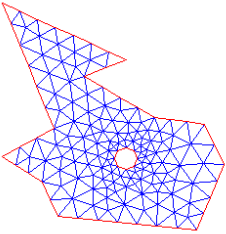
\includegraphics[width=0.34\textwidth]{assets/fig-2-1.png}
\figcaption{Rys. 2.1. \quad Przykładowy obszar symulacji podzielony nieregularną siatką trójkątną.}
\end{figure}

Rozwiązanie równania różniczkowego jest sumą przybliżonych rozwiązań znalezionych dla
wszystkich elementów siatki [2].
\begin{equation}
f(x,y)=\sum_{i=1}^{n}f_i(x,y). \tag{2.11}
\end{equation}
W najprostszym przypadku funkcje $f_i(x,y)$ mają postać wielomianów pierwszego stopnia dwóch
zmiennych przestrzennych:
\begin{equation}
f_i(x,y)=a+bx+cy. \tag{2.12}
\end{equation}
Znalezienie współczynników $a$, $b$, $c$ wymaga rozwiązania układu trzech równań liniowych z trzema
niewiadomymi, których współczynnikami są kombinacje położeń $(x_{iw},y_{iw})$ poszczególnych punktów
węzłowych elementu oraz rozwiązań zadanego równania różniczkowego w tych punktach. Postać
macierzową układu równań przedstawiono poniżej.
\begin{equation}
\begin{bmatrix}
f_{1w}\\ f_{2w}\\ f_{3w}
\end{bmatrix}
=
\begin{bmatrix}
1&x_{1w}&y_{1w}\\
1&x_{2w}&y_{2w}\\
1&x_{3w}&y_{3w}
\end{bmatrix}
\begin{bmatrix}
a\\ b\\ c
\end{bmatrix}. \tag{2.13}
\end{equation}
Tym samym macierz współczynników $a$, $b$, $c$ dana jest jako
\begin{equation}
\begin{bmatrix}
a\\ b\\ c
\end{bmatrix}
=
\begin{bmatrix}
1&x_{1w}&y_{1w}\\
1&x_{2w}&y_{2w}\\
1&x_{3w}&y_{3w}
\end{bmatrix}^{-1}
\begin{bmatrix}
f_{1w}\\ f_{2w}\\ f_{3w}
\end{bmatrix}. \tag{2.14}
\end{equation}
Metody numerycznego szukania wartości $f_1$, $f_2$, $f_3$ ściśle zależą od typu rozwiązywanego równania
różniczkowego.

\subchaptertitle{2.3. Równanie różniczkowe typu eliptycznego i metoda jego przybliżonego rozwiązywania}

Postać równania różniczkowego typu eliptycznego opisuje równanie (2.15), gdzie $f$ to funkcja
szukana na obszarze $\Omega$, zaś $a$, $b$ i $c$ są współczynnikami równania.
\begin{equation}
-\nabla\cdot(c\nabla f)+af=b. \tag{2.15}
\end{equation}
Wartość $f$ na brzegu obszaru $\Omega$ (dalej: $\partial\Omega$) określają warunki typu (2.16a) Dirichleta lub
(2.16b) Neumana.
\begin{align}
hf &= r, \tag{2.16a}\\
\mathbf n(c\nabla f)+qf &= g. \tag{2.16b}
\end{align}
Wielkości $h$, $r$ i $q$ to kolejne współczynniki równań, zaś $\mathbf n$ to wektor normalny do $\partial\Omega$. W przypadku
dwuwymiarowego wektorowego równania falowego, warunki brzegowe dobierane są tak, by
możliwie jak najlepiej uniknąć powstawania odbić na granicy obszaru symulacji. Tego problemu w
znacznej mierze można uniknąć stosując PML (idealnie dopasowana warstwa, ang. Perfectly
Matched Layer), o czym traktuje rozdział 2.4.

Równanie (2.15) mnoży się przez funkcję próbkującą $v$ i całkuje stronami na obszarze $\Omega$,
otrzymując równanie (2.17), a następnie całkuje przez części, doprowadzając je do postaci
przedstawionej w (2.18) [3,4].
\begin{align}
\int_\Omega\left((-\nabla\cdot c\nabla f)v+auf\right)\,dx &= \int_\Omega bv\,dx, \tag{2.17}\\
\int_\Omega\left((c\nabla f)\cdot\nabla v+afv\right)\,dx-\int_{\partial\Omega}(-qf+g)v\,ds &= \int_\Omega bv\,dx. \tag{2.18}
\end{align}
W dalszej kolejności, powyższe równanie zapisuje się w tzw. postaci słabej, zaś jego rozwiązanie
nosi nazwę rozwiązania słabego. Szukane są funkcje $f$ spełniające (2.19) dla wszystkich $v$.
\begin{equation}
\int_\Omega\left((c\nabla f)\cdot\nabla v+afv-bv\right)\,dx-\int_{\partial\Omega}(-qf+g)v\,ds=0. \tag{2.19}
\end{equation}
Funkcje $f$ i $v$ należą do tej samej przestrzeni $V$. Należy wybrać skończeniewymiarową
podprzestrzeń $V'\subset V$, której wymiar $\dim V'$ określa liczbę punktów węzłowych, do której należeć
będzie zbiór funkcji próbkujących $v_i$, tworzących bazę. Wymiar $V'$ stanowi o dokładności wyniku
obliczeń. Poszukiwane rozwiązanie problemu jest elementem podprzestrzeni leżącym najbliżej
wyniku rozwiązania słabego w sensie normy $||r||$, której postać podana jest poniżej.
\begin{equation}
||r||=\int_\Omega(c|f|^2+af^2)\,dx+\int_{\partial\Omega}qf^2\,ds. \tag{2.20}
\end{equation}
$f(x)$ można następnie rozwinąć w szereg, otrzymując przybliżone rozwiązanie
\begin{equation}
f(x)\approx\sum_{j=1}^{\dim V'}F_jv_j(x). \tag{2.21}
\end{equation}
Wstawienie powyższego wzoru do zdyskretyzowanego równania (2.18) daje poniższy układ
równań:
\begin{equation}
\begin{aligned}
\sum_{j=1}^{\dim V'}\bigg(&\int_\Omega\left((c\nabla v_j)\cdot\nabla v_j+av_jv_i\right)\,dx
+\int_{\partial\Omega}qv_jv_i\,ds\bigg)F_j \\
&=\int_\Omega bv_i\,dx+\int_{\partial\Omega}gv_i\,ds,\quad i=1,\ldots,\dim V'.
\end{aligned}
\tag{2.22}
\end{equation}
Wielkość (2.23a) określana jest mianem macierzy sztywności, zaś wielkość (2.23b) -- macierzy
masy. Nazwy te wynikają ze stosowalności powyższej metody do rozwiązywania problemów z
dziedziny statyki.
\begin{align}
K_{i,j} &= \int_\Omega(c\nabla v_j)\cdot\nabla v_i\,dx, \tag{2.23a}\\
M_{i,j} &= \int_\Omega av_jv_i\,dx. \tag{2.23b}
\end{align}
Otrzymany układ równań postaci $AF=B$ daje rozwiązania równania różniczkowego typu
eliptycznego dla wszystkich punktów węzłowych siatki. Szersze informacje na temat sposobu
przybliżonego znajdywania rozwiązań równań różniczkowych przedstawione są w [3,4].

\subchaptertitle{2.4. Warunki brzegowe PML}

Poważnym problemem napotykanym podczas wykonywania symulacji
elektromagnetycznych są odbicia propagujących się fal od brzegów obszaru symulacji, wynikające
z niedoskonałości zastosowanych warunków brzegowych. Wynikiem bywa poważne zaburzenie
otrzymanych rezultatów. W celu uniknięcia tego problemu, wprowadza się nieodbijającą i stratną
warstwę, noszącą nazwę PML (idealnie dopasowana warstwa, ang. Perfectly Matched Layer) [5].

\begin{figure}[H]\centering
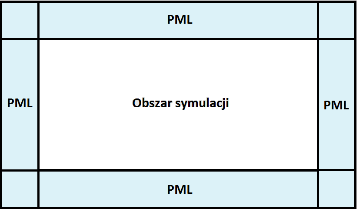
\includegraphics[width=0.56\textwidth]{assets/fig-2-2.png}
\figcaption{Rys. 2.2. \quad Schemat układu otoczonego warstwą PML.}
\end{figure}

Dla fali padającej prostopadle, warunkiem braku odbić na granicy ośrodków jest równość
impedancji $\eta=\sqrt{\mu/\epsilon}$.
\begin{equation}
\sqrt{\frac{\mu_0\mu_1}{\epsilon_0\epsilon_1}}=\sqrt{\frac{\mu_0\mu_2}{\epsilon_0\epsilon_2}}. \tag{2.24}
\end{equation}

Uogólnieniem tego warunku na przypadek padania ukośnego jest sztucznie wprowadzony
obszar o specjalnie dobranych, anizotropowych przenikalnościach $\epsilon$ i $\mu$. PML nie należy do obszaru
rozpatrywanego zagadnienia i jest niefizyczny. Materiały o właściwościach zbliżonych do idealnie
dopasowanej warstwy można jednakże uzyskać w postaci struktur wielowarstwowych [6].
Ostatecznie, wprowadzając macierz
\begin{equation}
S=\begin{bmatrix}s^{-1}&0\\0&s\end{bmatrix}, \tag{2.25}
\end{equation}
$s=1+\alpha i$, gdzie $\alpha$ jest dowolnie wybraną liczbą rzeczywistą, dwuwymiarowe wektorowe równania
falowe dla materiałów niemagnetycznych w obszarach PML dla polaryzacji TE i TM na granicy
poziomej obszaru symulacji będą miały postać kolejno (2.26a) i (2.26b), zaś w obszarach na
granicy pionowej (2.27a) i (2.27b).
\begin{align}
-\nabla\cdot(S\nabla E_z)-sk_0^2\epsilon_zE_z &= 0, \tag{2.26a}\\
-\nabla\cdot(S\epsilon^{-1}\nabla H_z)-sk_0^2H_z &= 0, \tag{2.26b}\\
-\nabla\cdot(S^{-1}\nabla E_z)-sk_0^2\epsilon_zE_z &= 0, \tag{2.27a}\\
-\nabla\cdot(S^{-1}\epsilon^{-1}\nabla H_z)-sk_0^2H_z &= 0, \tag{2.27b}
\end{align}
gdzie operator $\nabla$ ograniczony jest do dwóch wymiarów.
Równania te zmodyfikować można także dla obszarów narożnych, jednakże zastosowanie jednego
z powyższych również daje zadowalające rezultaty.

Przykład zastosowania idealnie dopasowanej warstwy przedstawiono na Rys. 2.3.
Rozważono dyfrakcję fali elektromagnetycznej o polaryzacji TE na cienkiej szczelinie wyciętej w
materiale będącym idealnym przewodnikiem. Dzięki zastosowaniu warunków brzegowych PML,
można zaobserwować brak powstawania odbić. Poniższy wynik otrzymano używając metody FEM.

\begin{figure}[H]\centering
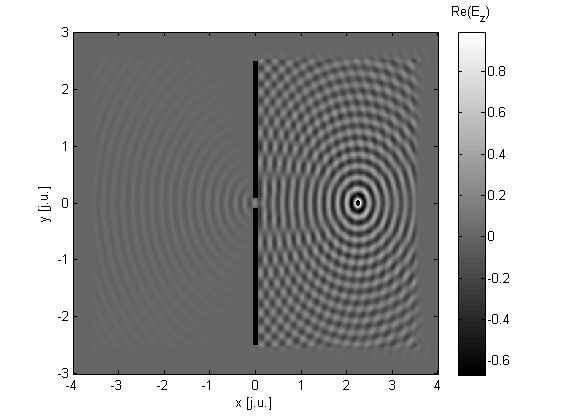
\includegraphics[width=0.58\textwidth]{assets/fig-2-3.png}
\figcaption{Rys. 2.3. \quad Dyfrakcja fali elektromagnetycznej na cienkiej szczelinie.}
\end{figure}

\subchaptertitle{2.5. Kryształy fotoniczne}

Kryształem nazywa się periodyczną strukturę, złożoną z atomów bądź molekuł. Sposób
rozmieszczenia tych komponentów definiuje rodzaj sieci krystalicznej układu. Charakterystyczną
właściwością kryształów jest możliwość występowania tzw. przerwy wzbronionej. Oznacza to, iż
dla pewnych wartości energii i pędu, elektron nie może poruszać się w takiej strukturze. W
przypadku, kiedy w określonym zakresie energii propagacja nie jest możliwa w żadnym kierunku,
przerwę nazywa się całkowitą, w przeciwnym razie nazywana jest częściową. Przykładem
występowania całkowitej przerwy wzbronionej jest struktura pasmowa półprzewodników, w
których rozdziela ona pasmo walencyjne od pasma przewodnictwa.

Analogiczną strukturą w optyce jest kryształ fotoniczny. Jest to periodyczna struktura
złożona z materiałów dielektrycznych, różniących się między sobą przenikalnością elektryczną.
Okres takiego układu jest porównywalny z długością fali, dla której ma on spełniać swoje funkcje.
Ze względu na kierunki okresowości, wyróżnia się kryształy jedno-, dwu- i trójwymiarowe.

\begin{figure}[H]\centering
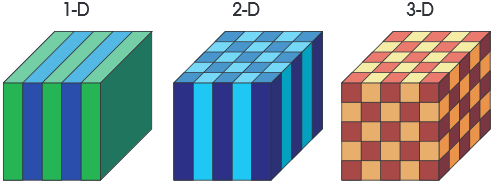
\includegraphics[width=0.66\textwidth]{assets/fig-2-4.png}
\figcaption{Rys. 2.4. \quad Schemat jedno-, dwu- i trójwymiarowego kryształu fotonicznego. Różnice w
kolorach symbolizują materiały o różnych wartościach przenikalności elektrycznej [7].}
\end{figure}

Podobnie jak w zwykłych kryształach (czy generalnie -- ośrodkach periodycznych), mody
kryształów fotonicznych mają postać fal Blocha. Zdarza się również, iż promieniowanie
elektromagnetyczne o określonych częstościach nie może rozchodzić się w strukturze. Mówi się
wtedy o fotonicznej przerwie wzbronionej. Jeśli, dla danego zakresu częstości, przerwa występuje
dla wszystkich polaryzacji i kierunków propagacji, nazywa się ją całkowitą, w przeciwnym zaś
wypadku -- częściową.

Możliwość selektywnej propagacji światła pozwala na tworzenie struktur o ciekawych
właściwościach optycznych, jak np. zwierciadła odbijające promieniowanie elektromagnetyczne o
określonym zakresie długości fali, materiały o prawie zerowej prędkości grupowej („spowalnianie”
światła), przeciwnych wartościach prędkości grupowej i fazowej (wsteczna propagacja), czy
materiały, na granicy których występuje ujemne załamanie. Inną możliwością jest tworzenie
falowodów opartych na kryształach fotonicznych. Do struktury wprowadzany jest defekt liniowy,
tworzony poprzez usunięcie rzędu lub kilku rzędów dielektrycznych słupków umieszczonych w
homogenicznej matrycy. W zakresie fotonicznej przerwy wzbronionej pojawia się mod defektowy,
pozwalający na propagację promieniowania elektromagnetycznego wzdłuż powstałego falowodu.
Zaletą takiej struktury jest znacznie niższa stratność np. w zakresie światła widzialnego, w
porównaniu do falowodów metalicznych.

\newpage
\subchaptertitle{2.6. Siatki dyfrakcyjne}

Siatka dyfrakcyjna jest to periodyczny układ szczelin (apertur) bądź przeszkód, powodujący
zmiany natężenia, fazy (lub obydwu jednocześnie) fali przechodzącej lub odbitej. Wyróżnia się dwa
podstawowe typy siatek: amplitudowe oraz fazowe. W pierwszym przypadku światło napotyka
naprzemiennie na przezroczyste i nieprzezroczyste obszary, przez co następuje modulacja
amplitudy. W drugim przypadku różnica dróg optycznych, wynikająca z karbowania
przezroczystych elementów, powoduje modulację fazy. Jeżeli karbowana siatka dyfrakcyjna nie jest
miejscami całkowicie przezroczysta, mamy do czynienia z modulacją zarówno amplitudową, jak i
fazową.

Dla fali padającej prostopadle na siatkę transmisyjną, wprowadzić można równanie
\begin{equation}
\Lambda\sin\theta=m\lambda, \tag{2.28}
\end{equation}
wiążące okres siatki $\Lambda$, kąt $\theta$, pod jakim obserwuje się maksima natężeń oraz długość fali $\lambda$. $m$ jest
liczbą całkowitą, indeksującą rząd ugięcia. Powyższe równanie uogólnić można dla padania
skośnego [8]:
\begin{equation}
\Lambda(\sin\theta_m-\sin\theta_i)=m\lambda. \tag{2.29}
\end{equation}
$\theta_i$ jest kątem, pod jakim fala pada na strukturę, zaś $\theta_m$ to kąt, pod jakim obserwuje się $m$-ty rząd
ugięcia.

\begin{figure}[H]\centering
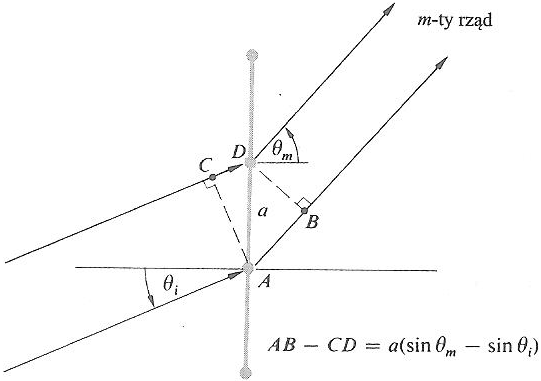
\includegraphics[width=0.64\textwidth]{assets/fig-2-5.png}
\figcaption{Rys. 2.5. \quad Schemat skośnego padania promieniowania elektromagnetycznego na transmisyjną
siatkę dyfrakcyjną [8].}
\end{figure}

Powyższe zależności mówią o tym, iż dla danej długości fali i określonego okresu siatki
dyfrakcyjnej, istnieje skończona liczba rzeczywistych rzędów ugięcia. Wiadomo, iż w dwóch
wymiarach zachodzi zależność
\begin{equation}
k_x^2+k_y^2=k_0^2n^2, \tag{2.30}
\end{equation}
gdzie $n$ jest współczynnikiem załamania ośrodka zewnętrznego. Jednocześnie, dla fali ugiętej na
układzie o periodyczności w kierunku $x$, wektor $k_x$ zachowany jest z dokładnością do
wielokrotności $2\pi/\Lambda$:
\begin{equation}
k_x^{(0)}=k_x^{(i)}+\frac{2\pi m}{\Lambda}, \tag{2.31}
\end{equation}
gdzie indeks (i) odpowiada fali padającej, zaś (0) opuszczającej siatkę.
Tym samym, dla dużych $m$, $|k_x^{(0)}|>k_0n$, toteż $k_y^{(0)}=\sqrt{k_0^2n^2-(k_x^{(0)})^2}$ przyjmuje wartości urojone.
Mamy wówczas do czynienia z ewanescentnymi, zanikającymi wykładniczo, rzędami ugięcia.

W przypadku siatek dyfrakcyjnych złożonych z kilku układów elementów o różnym okresie
periodyczności, liczba rzeczywistych rzędów ugięcia będzie zależeć od kierunku, z jakiego taka
struktura jest oświetlana. Zostało to pokazane w symulacjach, których wyniki zamieszczono w
podrozdziale 3.2.

\newpage
\chaptertitle{Rozdział 3. Wyniki symulacji}

W tym rozdziale zaprezentowano samodzielnie przeprowadzone symulacje. Wykorzystano metodę
elementów skończonych (pakiet „PDE Toolbox” firmy MathWorks), której wyniki porównano z
wybranymi rezultatami otrzymanymi metodą różnic skończonych w dziedzinie czasu [9] (program
MEEP [10]). W celu znalezienia struktury pasmowej kryształów fotonicznych, użyto programu
MPB -- MIT Photonic Bands [11], bazującego na metodzie fal płaskich.

\subchaptertitle{3.1. Propagacja światła w kryształach fotonicznych}

Rozpatrywano dwuwymiarowe kryształy fotoniczne o dwóch typach sieci: kwadratowej
oraz trójkątnej.

\begin{figure}[H]\centering
\begin{minipage}{0.33\textwidth}\centering
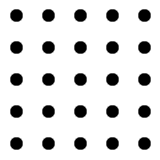
\includegraphics[width=0.85\linewidth]{assets/fig-3-1a.png}
\end{minipage}\hspace{0.8cm}
\begin{minipage}{0.33\textwidth}\centering
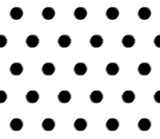
\includegraphics[width=0.85\linewidth]{assets/fig-3-1b.png}
\end{minipage}
\figcaption{Rys. 3.1. \quad Schematy dwuwymiarowych sieci krystalicznych: kwadratowej (z lewej) oraz
trójkątnej (z prawej).}
\end{figure}

Każdy z czarnych elementów na powyższym rysunku jest dielektrycznym słupkiem o
promieniu $0,2a$ (gdzie $a$ jest okresem sieci) i $n_1=1,7865$, co jest współczynnikiem załamania
szafiru (Al$_2$O$_3$) dla fali elektromagnetycznej o długości 400 nm [12]. Umieszczono je w materiale o
$n_2=1$, co z dobrą dokładnością można uznać za współczynnik załamania powietrza (w istocie jest
to współczynnik załamania próżni).

Struktury pasmowe wyznaczane były dla określonego, uprzednio zdefiniowanego,
współczynnika załamania. Jednakże, ze względu na dyspersję, faktycznie zmienia się on wraz ze
zmianą długości fali [13]. W związku z tym, modelowanie przeprowadzano dla uprzednio
wspomnianej fali o długości 400 nanometrów, zaś zmiany w częstości (wyrażonej w
bezwymiarowych jednostkach $2\pi c/a$) wprowadzano poprzez modyfikację rozmiarów kryształu, a
w szczególności wartości $a$.

Na Rys 3.2. pokazano wykres pasmowy, otrzymany dla światła o polaryzacji TE oraz TM w
krysztale fotonicznym o kwadratowym typie sieci. Dla żadnej z wymienionych polaryzacji nie
obserwuje się fotonicznej przerwy wzbronionej. Oznacza to, iż promieniowanie
elektromagnetyczne może propagować się w takiej strukturze dla wszystkich częstości, dla których
określono strukturę pasmową. Poprzez wycięcie jednego rzędu dielektrycznych słupków,
otrzymano falowód, a następnie, metodą elementów skończonych, zasymulowano rozchodzenie się
w nim światła.

\begin{figure}[H]\centering
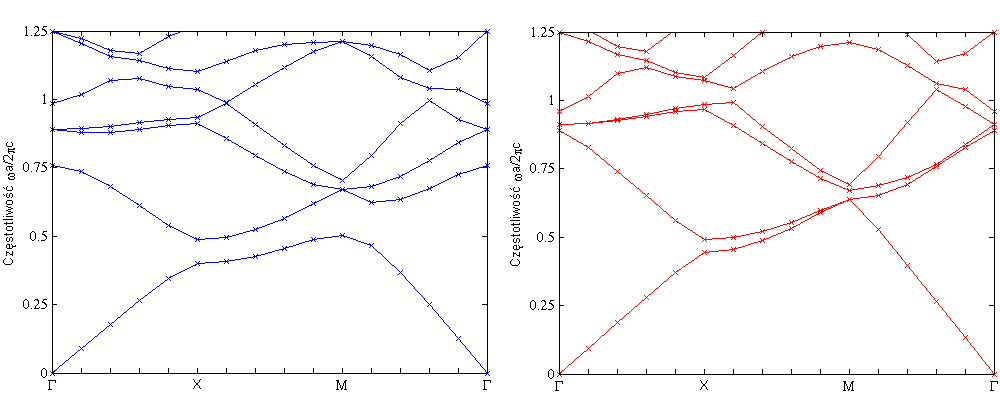
\includegraphics[width=0.88\textwidth]{assets/fig-3-2.png}
\figcaption{Rys. 3.2. \quad Struktura pasmowa kryształu o sieci kwadratowej, polaryzacja TE (lewy wykres),
polaryzacja TM (prawy wykres).}
\end{figure}

Rys. 3.3.-3.5. obrazują wyniki symulacji uzyskane dla powyższego przypadku dla trzech
różnych częstości promieniowania. W każdym przypadku, pole elektromagnetyczne wprowadzono
do układu dzięki zastosowaniu źródła sztywnego, znajdującego się w pobliżu rozpatrywanej
struktury. Symulacje przeprowadzono dla polaryzacji TE. Przedstawiono zarówno część
rzeczywistą pola $E_z$ fali, jak i jego fazę. Podobnie, jak zilustrowano to schematycznie na Rys. 2.2,
zewnętrzny obszar symulacji stanowi PML. Wszystkie symulacje propagacji promieniowania
elektromagnetycznego zostały przeprowadzone przy użyciu metody FEM, chyba, że w podpisie
zaznaczono inaczej.

\twopanel{assets/fig-3-3a.png}{assets/fig-3-3b.png}{Rys. 3.3. \quad Propagacja fali EM w krysztale fotonicznym o sieci kwadratowej z defektem
liniowym.}{a) Pole chwilowe $E_z$, b) faza pola $E_z$ dla $\omega=0,20\,2\pi c/a$.}

\twopanel{assets/fig-3-4a.png}{assets/fig-3-4b.png}{Rys. 3.4. \quad Propagacja fali EM w krysztale fotonicznym o sieci kwadratowej z defektem
liniowym.}{a) Pole chwilowe $E_z$, b) faza pola $E_z$ dla $\omega=0,45\,2\pi c/a$.}

\twopanel{assets/fig-3-5a.png}{assets/fig-3-5b.png}{Rys. 3.5. \quad Propagacja fali EM w krysztale fotonicznym o sieci kwadratowej z defektem
liniowym.}{a) Pole chwilowe $E_z$, b) faza pola $E_z$ dla $\omega=0,70\,2\pi c/a$.}

Powyższe symulacje potwierdzają, iż dla wybranych częstości, światło propaguje się w
rozpatrywanej strukturze.

Analogicznie, wyznaczono strukturę pasmową kryształu fotonicznego o sieci trójkątnej i
zobrazowano ją na Rys. 3.9. Dla polaryzacji TE, obserwuje się przerwę wzbronioną w zakresie
częstości $\omega a/2\pi c$ od ok. 0,48 do ok. 0,55. Została ona zaznaczona kolorem żółtym. W przypadku
polaryzacji TM, przerwy nie zaobserwowano. W związku z tym, podobnie jak dla sieci
kwadratowej, przeprowadzając symulacje skupiono się jedynie na pierwszej z tych polaryzacji.

\begin{figure}[H]\centering
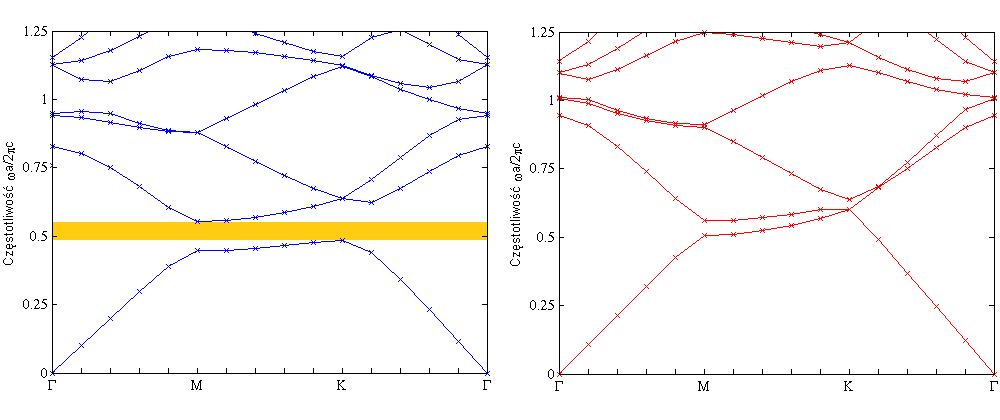
\includegraphics[width=0.88\textwidth]{assets/fig-3-6.png}
\figcaption{Rys. 3.6. \quad Struktura pasmowa kryształu o sieci trójkątnej, polaryzacja TE (lewy wykres),
polaryzacja TM (prawy wykres).}
\end{figure}

Wyznaczenie struktury pasmowej dla falowodu, powstałego przez usunięcie jednego rzędu
słupków, wskazuje na powstanie modu prowadzonego (wyszczególnionego kolorem zielonym),
leżącego wewnątrz przerwy wzbronionej kryształu, co widać na rysunku poniżej.

\begin{figure}[H]\centering
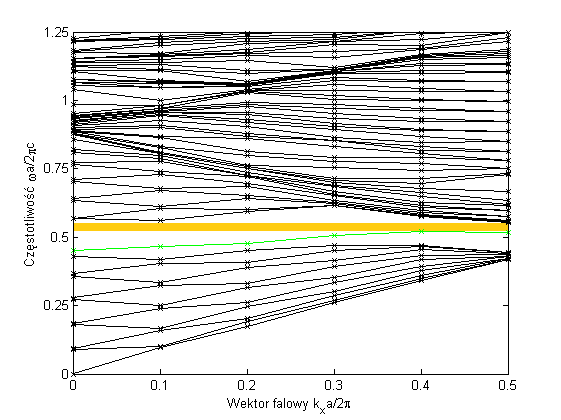
\includegraphics[width=0.66\textwidth]{assets/fig-3-7.png}
\figcaption{Rys. 3.7. \quad Struktura pasmowa kryształu o sieci trójkątnej z defektem liniowym.}
\end{figure}

Rys. 3.8.-3.10. obrazują rozchodzenie się w takim falowodzie promieniowania o
częstościach $\omega a/2\pi c$ kolejno: 0,20; 0,45 oraz 0,75. Nie leżą one w zakresie przerwy
wzbronionej, mają natomiast zobrazować różnice pomiędzy wynikami otrzymanymi dla sieci
kwadratowej oraz trójkątnej.

\twopanel{assets/fig-3-8a.png}{assets/fig-3-8b.png}{Rys. 3.8. \quad Propagacja fali EM w krysztale fotonicznym o sieci trójkątnej z defektem
liniowym.}{a) Pole chwilowe $E_z$, b) faza pola $E_z$ dla $\omega=0,20\,2\pi c/a$.}

\twopanel{assets/fig-3-9a.png}{assets/fig-3-9b.png}{Rys. 3.9. \quad Propagacja fali EM w krysztale fotonicznym o sieci trójkątnej z defektem
liniowym.}{a) Pole chwilowe $E_z$, b) faza pola $E_z$ dla $\omega=0,45\,2\pi c/a$.}

Rys. 3.8, otrzymany dla niskiej częstości, czyli dużej długości fali, jest zbieżny z
rezultatem otrzymanym dla takiej samej fali wejściowej podczas rozpatrywania układu o sieci
kwadratowej. Można wysnuć wniosek, iż w tym wypadku struktura kryształu nie wpływa na
sposób rozchodzenia się światła. Jest to potwierdzeniem faktu, iż stała sieci kryształu fotonicznego
powinna być porównywalna z długością fali, z którą kryształ ten ma oddziaływać, o czym
wspomniano w podrozdziale 2.5. Dopiero dla wyższych częstości różnice w propagacji zaczynają
być zauważalne. W niniejszej pracy nie modelowano jednakże propagacji światła dla bardzo
wysokich częstości, czyli dla fal o długościach o wiele mniejszych, niż stała sieci kryształu
fotonicznego.

\twopanel{assets/fig-3-10a.png}{assets/fig-3-10b.png}{Rys. 3.10 \quad Propagacja fali EM w krysztale fotonicznym o sieci trójkątnej z defektem liniowym.}{a) Pole chwilowe $E_z$, b) faza pola $E_z$ dla $\omega=0,70\,2\pi c/a$.}

W dalszej kolejności, wykonano modelowanie dla fali elektromagnetycznej o częstości z
zakresu modu prowadzonego. Łatwo zauważyć, iż światło propaguje się głównie wzdłuż defektu
liniowego, zaś w zasadzie nie obserwuje się rozchodzenia się w innych kierunkach. Zostało to
zobrazowane poniżej.

\twopanel{assets/fig-3-11a.png}{assets/fig-3-11b.png}{Rys. 3.11 \quad Propagacja fali EM w krysztale fotonicznym o sieci trójkątnej z defektem liniowym.}{a) Pole chwilowe $E_z$, b) faza pola $E_z$ dla $\omega=0,50\,2\pi c/a$.}

W celach porównawczych, symulację powtórzono metodą różnic skończonych w dziedzinie
czasu. Otrzymano porównywalny rezultat. Niewielkie różnice mogą wynikać z faktu, iż wynikiem
obliczeń jest pole chwilowe, jak również z faktu, iż w programie MEEP zastosowano inny typ
źródła, niebędący źródłem sztywnym, jak również inną aplitudę wejściową. Nie ma jednakże
wątpliwości, iż rezultaty otrzymane metodami FEM i FDTD są zgodne.

\begin{figure}[H]\centering
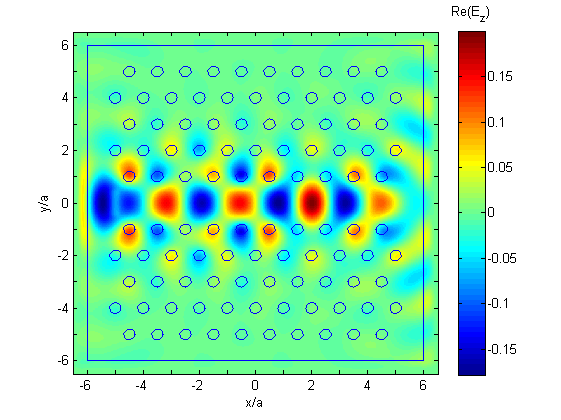
\includegraphics[width=0.48\textwidth]{assets/fig-3-12.png}
\figcaption{Rys. 3.12. Propagacja fali EM w krysztale fotonicznym o sieci trójkątnej z defektem liniowym.
Pole chwilowe $E_z$ dla $\omega=0,50\,2\pi c/a$. Symulacja wykonana metodą FDTD.}
\end{figure}

Wreszcie, dla częstości leżącej wewnątrz przerwy wzbronionej (wybrano wartość
$\omega=0,538\,\omega a/2\pi c$), obserwuje się zanik amplitudy fali wraz ze wzrostem odległości od źródła.
Wyniki symulacji przeprowadzonych metodą elementów skończonych są więc zbieżne z zakresami
fotonicznej przerwy wzbronionej i modu prowadzonego, wyznaczonymi programem MPB.

\twopanel{assets/fig-3-13a.png}{assets/fig-3-13b.png}{Rys. 3.13. \quad Propagacja fali EM w krysztale fotonicznym o sieci trójkątnej z defektem liniowym.}{a) Pole chwilowe $E_z$, b) faza pola $E_z$ dla $\omega=0,538\,2\pi c/a$.}

Podobnie jak w przypadku symulacji przeprowadzonych dla prowadzenia światła w
zlokalizowanym modzie defektowym, metoda różnic skończonych w dziedzinie czasu daje niemal
identyczne rezultaty, co metoda elementów skończonych, dla częstości leżącej wewnątrz
fotonicznej przerwy wzbronionej.

\begin{figure}[H]\centering
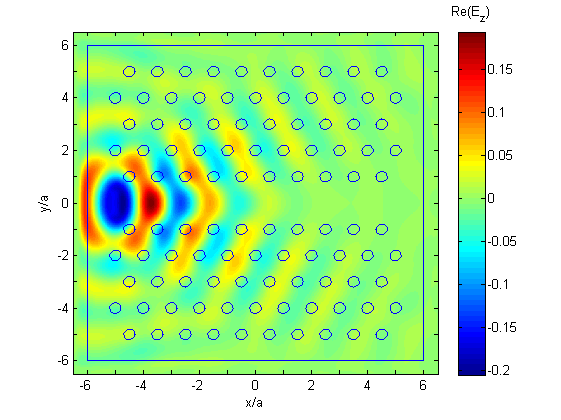
\includegraphics[width=0.48\textwidth]{assets/fig-3-14.png}
\figcaption{Rys. 3.14. Propagacja fali EM w krysztale fotonicznym o sieci trójkątnej z defektem liniowym.
Pole chwilowe $E_z$ dla $\omega=0,538\,2\pi c/a$. Symulacja wykonana metodą FDTD.}
\end{figure}

\newpage
\subchaptertitle{3.2. Elementy dyfrakcyjne o podwójnej periodyczności}
\begingroup\small

Elementy dyfrakcyjne o podwójnej periodyczności są to układy zbudowane z dwóch siatek
podfalowych o różnych okresach. Zgodnie z tym, co przedstawiono w rozdziale 2.6, liczba
rzeczywistych rzędów ugięcia zależy od kierunku, z jakiego światło pada na tak skonstruowaną
strukturę. Jednocześnie, możliwe jest zaobserwowanie niesymetrycznej transmisji promieniowania
elektromagnetycznego oraz usunięcie zerowego rzędu ugięcia [14].

W symulacjach przeprowadzonych na potrzeby tego rozdziału, rozpatrzono układy
zbudowane kolejno z idealnego przewodnika, chromu, złota oraz srebra. Ich schemat przedstawiono
na poniższym rysunku.

\begin{figure}[H]\centering
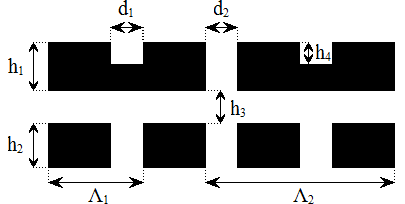
\includegraphics[width=0.58\textwidth]{assets/fig-3-15.png}
\figcaption{Rys. 3.15. \quad Schemat siatki dyfrakcyjnej o podwójnej periodyczności.}
\end{figure}

Zastosowano wymiary kolejno: $2\Lambda_1=\Lambda_2=533$ nm; $d_1=d_2=89$ nm ; $h_1=h_2=127$ nm; $h_3=89$ nm;
$h_4=63,5$ nm.

Poniższe symulacje zostały przeprowadzone metodą FEM dla fali elektromagnetycznej o
długości 400 nm. Zastosowano polaryzację TM. Wartości przenikalności elektrycznych dla
rozważanych metali zestawiono w tabeli.

\begin{table}[H]\centering
\caption*{\small Tabela 3.1 \quad Przenikalności elektryczne wybranych metali dla fal o długości 400 nm [15].}
\begin{tabular}{|p{0.29\textwidth}|p{0.29\textwidth}|p{0.29\textwidth}|}
\hline
& \centering $\epsilon_1$ & \centering\arraybackslash $\epsilon_2$\\
\hline
Srebro & -4,422 & 0,210\\
\hline
Złoto & -1,658 & 5,735\\
\hline
Chrom & -4,055 & 11,480\\
\hline
\end{tabular}
\end{table}

Przenikalności $\epsilon_1$ oraz $\epsilon_2$ wnoszą wkład w zespoloną przenikalność elektryczną
\begin{equation}
\tilde\epsilon=\epsilon_1+i\epsilon_2. \tag{3.1}
\end{equation}
Do emisji fal kulistych użyto pięciu źródeł sztywnych, których centra znajdowały się nad
szczelinami siatki.

Rys. 3.16. obrazuje transmisję światła przez strukturę, w której siatka dyfrakcyjna
zbudowana jest z idealnego przewodnika. Dla fali elektromagnetycznej padającej z góry widać dwa
rzędy ugięcia: -1 i 1. W przypadku padania z drugiej strony, obserwuje się jedynie zerowy rząd
ugięcia, co jest to zgodne z teorią przedstawioną w podrozdziale 2.6.

\newpage
\twopanel{assets/fig-3-16a.png}{assets/fig-3-16b.png}{Rys. 3.16. \quad Siatka z idealnego przewodnika,}{a) padanie z góry, b) padanie z dołu.}

Zastosowanie fal kulistych spowodowało, iż w zerowym rzędzie ugięcia obserwuje się delikatne
odchylenie od kąta 0° w stosunku do normalnej względem kierunku periodyczności struktury.
Wynika to ze wzoru 2.29.

Porównywalne rezultaty otrzymano w przypadku symulacji przeprowadzonych dla chromu.
Obserwuje się zwiększoną transmisję w porównaniu z idealnym przewodnikiem, jednakże można
wysnuć wniosek, iż z trzech rozpatrywanych metali, ten jest do niego najbardziej podobny.

\twopanel{assets/fig-3-17a.png}{assets/fig-3-17b.png}{Rys. 3.17. \quad Siatka z chromu,}{a) padanie z góry, b) padanie z dołu.}

W przypadku zastosowania złota, obserwuje się wzmożoną transmisję przez strukturę.
Można zauważyć wnikanie światła w elementy układu. Dla symulacji, w której fala
elektromagnetyczna padała z góry, wyraźnie można dostrzec trzy rzędy ugięcia.

\newpage
\twopanel{assets/fig-3-18a.png}{assets/fig-3-18b.png}{Rys. 3.18. \quad Siatka ze złota,}{a) padanie z góry, b) padanie z dołu.}

Ciekawe rezultaty otrzymano dla układu zbudowanego ze srebra, dla którego transmisja
promieniowania elektromagnetycznego okazała się szczątkowa bez względu na kierunek jego
padania.

\twopanel{assets/fig-3-19a.png}{assets/fig-3-19b.png}{Rys. 3.19. \quad Siatka ze srebra,}{a) padanie z góry, b) padanie z dołu.}

\endgroup
\newpage
\chaptertitle{Rozdział 4. Podsumowanie}

Na potrzeby niniejszej pracy, przeprowadzono szereg symulacji dotyczących propagacji
światła w kryształach fotonicznych oraz elementach dyfrakcyjnych o podwójnej periodyczności.
Bazowano na metodzie elementów skończonych.

W przypadku kryształów fotonicznych, zaczęto od wyznaczenia ich struktury pasmowej, co
było możliwe dzięki posiłkowaniu się metodą fal płaskich, mającą zastosowanie w optycznych
układach periodycznych. Rozpatrzono dwa rodzaje sieci: kwadratową i trójkątną. Zachowanie
światła o określonej długości fali modelowano poprzez zmianę rozmiarów kryształu fotonicznego.
Sprawdzono, iż w niektórych tego typu strukturach, dla pewnych polaryzacji fali, w określonym
zakresie częstości, występuje fotoniczna przerwa wzbroniona. Pokazano również, iż poprzez
wprowadzenie defektów, możliwe staje się efektywne prowadzenie światła o częstości leżącej
wewnątrz takiej przerwy dzięki powstawaniu modu defektowego. Wybrane wyniki porównano
następnie z symulacjami przeprowadzonymi metodą różnic skończonych w dziedzinie czasu.

Dla elementów dyfrakcyjnych o podwójnej periodyczności wykazano, iż ilość
obserwowanych rzeczywistych rzędów ugięcia zależna jest w ogólności od kierunku oświetlania
struktury. Udowodniono też, iż znaczny wpływ na sposób działania układu ma materiał, z którego
jest on wykonany. W tym celu modelowanie przeprowadzono dla idealnego przewodnika, chromu,
złota oraz srebra. Dla idealnego przewodnika i chromu zauważono wiele podobieństw, w przypadku
złota obserwowano wzmożoną transmisję promieniowania elektromagnetycznego, zaś w przypadku
srebra -- nie obserwowano jej prawie w ogóle.

Pokazano, iż metoda elementów skończonych jest przydatnym narzędziem, mogącym służyć
do projektowania układów optycznych o charakterystycznych właściwościach. Pomocnicze użycie
narzędzi takich, jak metoda fal płaskich, znacząco ułatwiło zasymulowanie różnic w zachowaniu się
światła w zależności od rozmiarów struktury, czy materiału, z jakiego jest wykonana.
Udowodniono, iż niezwykle ważne w efektywnym projektowaniu nowych materiałów jest
połączenie kilku technik pozwalających określić właściwości struktury. Daje to możliwość łatwej
optymalizacji elementów optycznych, a także szansę na efektywne projektowanie nowych, bardziej
złożonych układów.

\newpage
\chaptertitle{Bibliografia}

\begin{enumerate}
\renewcommand{\labelenumi}{[\arabic{enumi}]}
\item D. J. Griffiths, \textit{Podstawy elektrodynamiki}, wyd. 2, Wydawnictwo Naukowe PWN (2005), str. 354-366
\item M. N. O. Sadiku, \textit{Numerical Techniques in Electromagnetics}, wyd. 2, CRC Press (2000), rozdział 6
\item C. Johnson, \textit{Numerical Solution of Partial Differential Equations by the Finite Element Method}, Cambridge University Press (1987)
\item R. E. Bank, \textit{PLTMG A Software Package for Solving Elliptic Partial Differential Equations}, User’s Guide 6.0, Society for Industrial and Applied Mathematics, Philadelphia, PA (1990)
\item J.P. Berenger, \textit{Perfectly Matched Layer (PML) for Computational Electromagnetics}. Morgan and Claypool, Los Altos (2007)
\item A. Pastuszczak, M. Stolarek, T. J. Antosiewicz i R. Kotyński, \textit{Multilayer metamaterial absorbers inspired by perfectly matched layers}, Optical and Quantum Electronics, DOI 10.1007/s11082-014-9986-z (2014)
\item J. D. Joannopoulos, S. G. Johnson, J. N. Winn i R. D. Meade, \textit{Photonic Crystals, Molding the Flow of Light}, wyd. 2, Princeton University Press (2008), str. 4
\item E. Hecht, \textit{Optyka}, wyd. 1, Wydawnictwo Naukowe PWN (2005), str. 479-482
\item A. Taflove, S. C. Hagness, \textit{Computational Electrodynamics: The Finite-Difference Time-Domain Method}, wyd. 3, Artech House (2005)
\item A. F. Oskooi, D. Roundy, M. Ibanescu, P. Bermel, J. D. Joannopoulos i S. G. Johnson, \textit{MEEP: A flexible free-software package for electromagnetic simulations by the FDTD method}, Computer Physics Communications \textbf{181}, str. 687--702 (2010)
\item S. G. Johnson i J. D. Joannopoulos, \textit{Block-iterative frequency-domain methods for Maxwell's equations in a planewave basis}, Optics Express \textbf{8}, str. 173-190 (2001)
\item I. H. Malitson i M. J. Dodge. \textit{Refractive Index and Birefringence of Synthetic Sapphire}, J. Opt. Soc. Am. \textbf{62}, 1405 (1972)
\item B. E. A. Saleh i M. C. Teich, \textit{Fundamentals of Photonics}, wyd. 2, Wiley-Interscience (2007), str. 173-174
\item M. Stolarek, D. Yavorskiy, R. Kotyński, C. J. Zapata Rodríguez, J. Łusakowski i T. Szoplik, \textit{Asymmetric transmission of terahertz radiation through a double grating}, Optics Letters \textbf{38}, str. 839-841 (2013)
\item P. B. Johnson i R. W. Christy. \textit{Optical Constants of the Noble Metals}, Physical Review \textbf{B 6}, str. 4370-4379 (1972)
\end{enumerate}

\end{document}
